\chapter{Strumenti numerici indicatori - parte V}

\begin{figure}[h]
    \centering
    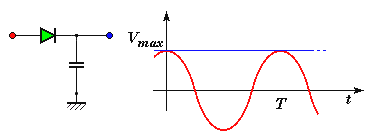
\includegraphics[scale = 2]{Come convertire da AC a DC.png}
\end{figure}

\newpage    

\section{Voltmetro numerico in AC}
\footnote{Slide della prof | SDME 4 Strumenti numerici indicatori - parte V | pag 3 \\  
Appunti | 2025-05-07 | pag 8}

In questo capitolo studieremo ed analizzeremo il voltmetro in AC (Accoppiato in alternata). \newline 

In particolare, il nostro focus sarà sui seguenti argomenti del voltmetro in AC: 

\begin{itemize}
    \item il valore efficace, in particolare il fattore di cresta 
    \item la misurazione del valore efficace
\end{itemize}

\newpage 

\begin{tcolorbox}
    È letteralmente la stessa slide del capitolo 13, quindi l'ho copiata
\end{tcolorbox}

\section{Valore efficace}
\footnote{Slide della prof | SDME 4 Strumenti numerici indicatori - parte III | pag  15, 23 \\  
Appunti | 2025-04-29 | pag 10} 

Un altro parametro molto importante è il valore efficace. \newline 

In un tempo pari ad un periodo T, una corrente alternata con valore efficace di 1 A che circola su di un resistore 
dissipa la stessa energia che sarebbe dissipata nello stesso tempo, da una corrente costante con intensità di 1 A. \newline 

Per dare questa definizione, la corrente alternata è periodica ed ha valore medio nullo. \newline 

In formule: 

{
    \Large 
    \begin{equation}
        I 
        = 
        \sqrt
        {
            \frac{1}{T}
            \int_{t_0}^{t_0 + T} 
            i^{2} (t) dt
        }
    \end{equation}
}

Anche se fisicamente non esiste, 
si è data anche la definizione di tensione efficace come: 

{
    \Large 
    \begin{equation}
        V 
        = 
        \sqrt
        {
            \frac{1}{T}
            \int_{t_0}^{t_0 + T} 
            v^{2} (t) dt
        }
    \end{equation}
}

\begin{tcolorbox}
Stare attenti alla nomenclatura: I e V con le lettere maiuscole intendono rispettivamente la corrente efficace e la tensione efficace    
\end{tcolorbox}

\newpage 

\section{La distribuzione in alternata}
\footnote{Slide della prof | SDME 4 Strumenti numerici indicatori - parte V | pag 5 \\  
Appunti | 2025-05-07 | pag 8}

L'introduzione della definizione di corrente efficace (e poi di conseguenza quella di tensione efficace) 
è stata dettata dalla necessità di passare dalla distribuzione in continua di energia elettrica alla distribuzione in alternata. \newline 

Come visualizzato dal seguente schema dell'architettura di una rete di distribuzione di energia in alternata: 

\begin{figure}[h]
    \centering
    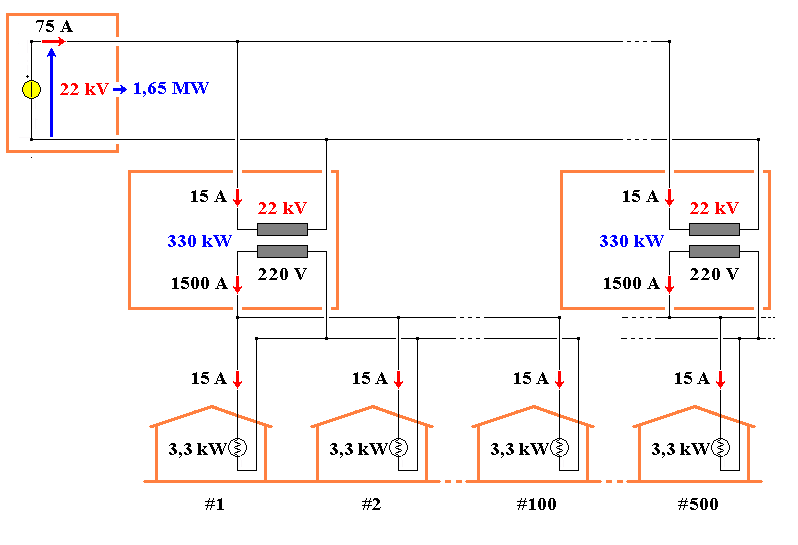
\includegraphics[scale = 1]{Rete di distribuzione di energia in alternata esempio.png}
\end{figure}

(partendo dal rettangolo aracione posto in alto a sinistra) una rete di distribuzione di energia in alternata consente di uscire dalla centrale con linee elettriche in alta tensione, 
e quindi, correnti relativamente ridotte e abbassare la tensione in vicinanza delle utenze finali mediante l'uso di trasformatori, per migliorare la sicurezza dell'impianto. \newline 

L'uso dei trasformatori richiede, inevitabilmente, il passaggio al regime alternato, perchè, come studiato nel corso di elementi di elettromagnetismo con il mitico Zappelli, 
le bobine dei primari e secondari di un trasformatore sono dei solenoidi, in cui legge caratteristica vale per una corrente alternata. \newline 

L'introduzione del valore efficace consente di esprimere la similitudine tra gli effetti energetici della corrente continua agli effetti energetici di quella alternata. \newline 

\newpage 

\subsection{La distribuzione in regime sinusoidale}
\footnote{Slide della prof | SDME 4 Strumenti numerici indicatori - parte V | pag 6 - 7 \\  
Appunti | 2025-05-07 | pag 8 - 9 | 2025-06-23 Ricevimento | pag 6 - 7}

Perché, tra tutte le forme possibili di regime alternato, è stato scelto quello sinusoidale? \newline 

I trasformatori lavorano producendo in uscita una grandezza ottenuta come derivata temporale della grandezza in ingresso. \newline 

La legge di Faraday: 

{
    \Large 
    \begin{equation}
        \begin{cases}
            fem_{indotta} = - \frac{\partial \Phi (t)}{\partial t}
            \\ 
            i_{indotta} = - \frac{1}{R} \cdot \frac{\partial \Phi (t)}{\partial t}
        \end{cases}
    \end{equation}
}

lega la tensione che si produce in una spira alla derivata nel tempo del flusso magnetico, che si concatena con la spira stessa. \newline 

Le uniche funzioni la cui propria derivata ha la stessa forma della funzione che viene derivata sono la sinusoide e l'esponenziale. \newline 

Consideriamo g(t) una funzione di una tensione data al primario di un trasformatore con rapporto 1:1 tra primario e secondario: 

{
    \Large 
    \begin{equation}
        g(t) = G_{max} \sin(\omega t)
    \end{equation}
}

dove $G_{max}$ è la tensione di picco di g(t) e $\omega$ è la pulsazione di g(t). \newline 

Derivando g(t) e applicando una uguaglianza trigonometrica: 

{
    \Large 
    \begin{equation}
        \begin{split}
            \frac{\partial g(t)}{\partial t}
            &= 
            \omega G_{max} \cos(\omega t)
            \\
            &= 
            \omega G_{max} \sin(\omega t + \frac{\pi}{2})
        \end{split}
    \end{equation}
}

Queste equazioni mostrano che, attraverso un trasformatore alimentato con un'onda sinusoidale, 
si ottiene ancora un'onda sinusoidale (a meno di uno sfasamento di $\frac{\pi}{2}$). \newline 

Questo concetto è ancora più importante pensando che nella rete di distribuzione si ha una "cascata" di trasformatori. \newline 

\newpage 

I trasformatori di grandi potenze, in uscita delle cabina primarie, riducono la tensione a kV (MT o MV): 

\begin{figure}[h]
    \centering
    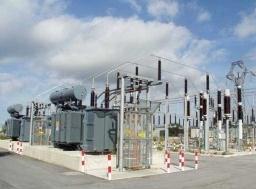
\includegraphics[scale = 2]{Foto di un trasformatore di grande potenza.png}
\end{figure}

\begin{tcolorbox}
Un esempio di trasformatore di grande potenza è quello presente alla Baraccola in Via Achille Grandi 44 in Ancona \\
\url{https://maps.app.goo.gl/EAHYg4zSwEkYsJy27}    
\end{tcolorbox}

L'energia passa dai trasformatori di grandi potenze alle cabine secondarie (da palo o in muratura): 

\begin{figure}[h]
    \centering
    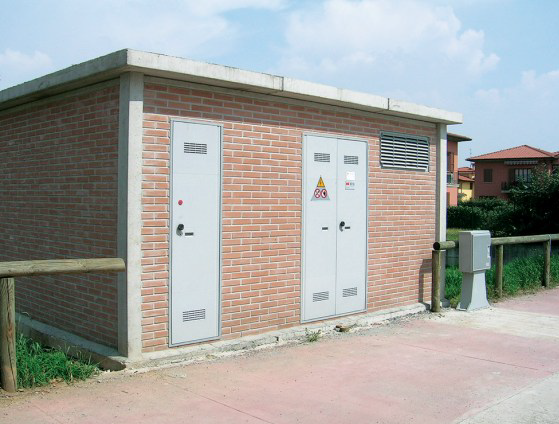
\includegraphics[scale = 0.8]{Foto cabina secondaria.png}
    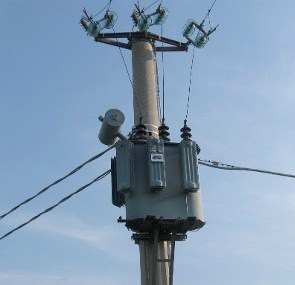
\includegraphics[scale = 1]{Foto palo di media tensione.png}
\end{figure}

con trasformatori (in resina o in olio per mantenere la temperatura costante e dissipare più facilmente il calore dei trasformatori, quindi delle bobine), 
che riducono ancora la tensione da valore efficace 30 kV a 230 V, con cui si alimentano le nostre utenze. \newline 

\begin{tcolorbox}
    Esempio di una cabina secondaria a media tensione è quella del McDonald's di Torrette di Ancona vicino al Coal in Via Tenna 24\\
    \url{https://maps.app.goo.gl/YvFRXkAVv1JjhkRdA}
\end{tcolorbox}

A casa sono presenti altri trasformatori di diverse dimensioni, 
dimensioni che dipendono dal carico da sostenere: possono essere grandi se devono alimentare una serie di frigoriferi, o possono essere di dimensioni ridotte se devono alimentare gli smartphone. \newline 

In generale, possiamo dire che la rete di distribuzione di energia è alquanto complessa, quindi se si possono semplificare i conti a monte è cosa buona e giusta. \newline 

\newpage 

\section{Misurazione del valore efficace (G) di una grandezza sinusoidale}
\footnote{Slide della prof | SDME 4 Strumenti numerici indicatori - parte V | pag 8 \\  
Appunti | 2025-05-07 | pag 9}

Per calcolare il valore efficace di una grandezza sinusoidale si possono implementare tre tipi di convertitori: 

\begin{itemize}
    \item convertitori e metodi di misura utilizzando la termometria (TRMS) a valore efficace 
    \item convertitori basati su misurazione indiretta (RMS) a quasi valore efficace 
    \item convertitori basati sul calcolo del valore medio del quadrato del segnale (TRMS)
\end{itemize}

\newpage 

\section{Carichi non lineari e regimi non sinusoidali}
\footnote{Slide della prof | SDME 4 Strumenti numerici indicatori - parte V | pag 9\\  
Appunti | 2025-05-07 | pag 9}

Grazie alla forte diffusione dei dispositivi digitali, 
un problema che ha comportato alla rete di distribuzione di energia è quello di "sporcarla", 
cioè aggiungere un rumore non lineare e non sinusoidale dovuto agli alimentatori switching. \newline 

Gli alimentatori switching sono composti da FET, che hanno il vantaggio di essere fisicamente di dimensioni compatte rispetto alle grosse bobine 
dei trasformatori tradizionali, ma i FET si comportano da interruttori aperti e chiusi in modo quasi istantaneo. \newline 

Quindi, da una tensione di distribuzione della rete tendenzialmente sinusoidale, questa ultima sarà sporcata dai rumori dei dispositivi non lineari, non sinusoidali, 
dei dispositivi che utilizziamo ogni giorno in casa: 

\begin{figure}[h]
    \centering
    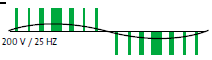
\includegraphics[scale = 2]{Tensione sinusoidale sporcata da alimentatori switching.png}
\end{figure}

\begin{tcolorbox}
    Se vuoi approfondire l'argomento: \\ 
    Come funzionano gli alimentatori switching AC/DC? - Risposte da cani by Video da cani \\ 
    \url{https://youtu.be/Qz2MioZEiBE?si=BkaENSF6yWXhJxeM}
\end{tcolorbox}

A causa di queste, e molte altre forme di onde, il gold standard è quello di misurare il valore efficace attraverso la termometria. \newline 

\newpage 

\section{Valore efficace e la misura per termometria}
\footnote{Slide della prof | SDME 4 Strumenti numerici indicatori - parte V | pag 10\\  
Appunti | 2025-05-07 | pag 9 - 10} 

Riportiamo la definizione di valore efficace della corrente I: 

"In un tempo pari ad un periodo T, una corrente alternata con valore efficace di 1 A che circola su di un resistore 
dissipa la stessa energia che sarebbe dissipata nello stesso tempo, da una corrente costante con intensità di 1 A." \newline 

Su questa definizione, sono basati gli strumenti ed i metodi di misura per termometria. \newline 

Come si può visualizzare dal seguente circuito: 

\begin{figure}[h]
    \centering
    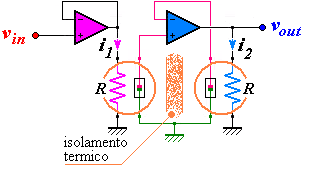
\includegraphics[scale = 1.5]{Misura per termometria circuito.png}
\end{figure}

(partendo da sinistra della figura) si fa circolare una corrente costante su una resistenza: 

{
    \Large 
    \begin{equation}
        i_1 (t) = \frac{v_{in}(t)}{R}
    \end{equation}
}

in modo da provocare, sull'altra resistenza (quella a destra) lo stesso riscaldamento che si ha su una resistenza identica 
percorsa dalla corrente $i_2$: 

{
    \Large 
    \begin{equation}
        \begin{split}
        v_{out} &= R \cdot i_2
        \\ 
        &\updownarrow 
        \\
        i_2 &= \frac{v_{out}}{R}
        \end{split}        
    \end{equation}
}

il cui valore efficace deve essere misurato. \newline 

In questa maniera si è applicata una conversione da TRMS a DC utilizzando la temperatura. \newline 

\newpage 

\subsection{Fluke 792A Transfer Standard}
\footnote{Slide della prof | SDME 4 Strumenti numerici indicatori - parte V | pag 11\\  
Appunti | 2025-05-07 | pag 10}

Uno strumento che applica la definizione di valore efficace è il Fluke 792A Transfer Standard: 

\begin{figure}[h]
    \centering
    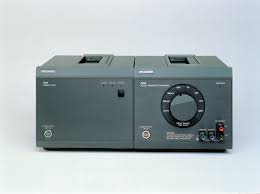
\includegraphics[scale = 1]{Fluke 792A Transfer Standard.jpg}
\end{figure}

Questo dispositivo è molto versatile perchè è utilizzabile sia con tensione in AC che in DC, ha un range di tensioni che va dai 2 mV a 1000V, 
per segnali da 10 Hz a 1 MHz e, nonostante tutta questa enorme versatilità, presenta solo $\pm 10$ ppm di incertezza. \newline 

Essendo uno strumento che sfrutta le proprietà della temperatura tra i due resistori uguali, ha bisogno di un warm up  time, che in questo caso è di 15 minuti 
(in gergo misuristico, si va a prendere un caffè poi si ritorna in laboratorio). \newline 

Il warm up time è necessario affinché i componenti possano superare i transitori termici. \newline 

\newpage 

\section{Fattore di cresta}
\footnote{Slide della prof | SDME 4 Strumenti numerici indicatori - parte V | pag 12\\  
Appunti | 2025-05-07 | pag 10 | 2025-05-09 | pag 2} 

Cambiando prospettiva e andando a considerare strumenti nettamente molto più economici del Transfer Standard per la misura del valore efficace, 
dobbiamo introdurre un nuovo parametro. \newline 

Esso ci consente di stimare il valore efficace mediante una misura indiretta, che va a valutare il fattore di cresta. \newline 

Il fattore di cresta di un segnale periodico è il rapporto fra il massimo valore istantaneo (o anche detto valore di picco) ed il valore efficace. \newline 

Come scritto nel capitolo 13, il valore di corrente efficace I  partendo da una corrente puramente sinusoidale e con sfasamento nullo: 

{
    \Large 
    \begin{equation}
        I = \frac{I_{pk}}{\sqrt{2}}
    \end{equation}
}

dove $I_{pk}$ è il valore di picco di i(t). \newline 

Il fattore di cresta è proprio $\sqrt{2}$. \newline 


\newpage 

\section{Convertitore RMS / DC a misura indiretta (tensione di picco)}
\footnote{Slide della prof | SDME 4 Strumenti numerici indicatori - parte V | pag 13\\  
Appunti | 2025-05-07 | pag 11 | 2025-05-09 | pag 3} 

Idealmente, dato un segnale di ingresso sinusoidale e periodico, 
possiamo rivelare la tensione massima del segnale di ingresso con il seguente circuito: 

\begin{figure}[h]
    \centering
    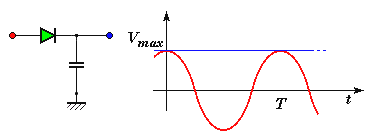
\includegraphics[scale = 1.5]{Diodo e condensatore per fattore di cresta.png}
\end{figure}

Con questo semplice circuito (figura a sinistra), 
la tensione massima ($V_{max}$ di colore blu nella figura a destra e pin blu nella figura del circuito) rimane costante nel tempo, 
rispetto al segnale sinusoidale periodico di ingresso (nella figura a destra di colore rosso e pin rosso nella figura del circuito). \newline 


\newpage 

\subsection{RMS / DC a valore di picco: modello completo}
\footnote{Slide della prof | SDME 4 Strumenti numerici indicatori - parte V | pag 14\\  
Appunti | 2025-05-09 | pag 3 - 4} 

Passando dal modello ideale visualizzato nella sezione precedente al modello reale, 
dovremo considerare le resistenze parassite dei componenti. \newline 

Quindi, da una tensione $V_{max}$ costante in uscita con ingresso una tensione sinusoidale periodica, 
avremo questo andamento:  

\begin{figure}[h]
    \centering
    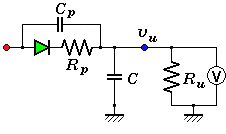
\includegraphics[scale = 1.5]{Diodo e condensatore per fattore di cresta circuito reale.png}
    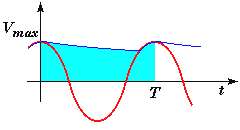
\includegraphics[scale = 1.5]{Andamento non sinusoidale di un circuito con diodo e condensatore reale.png}
\end{figure}

Confrontando il circuito reale con quello ideale: 

\begin{figure}[h]
    \centering
    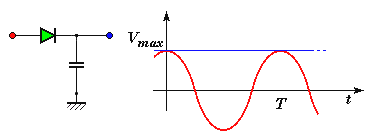
\includegraphics[scale = 1.5]{Diodo e condensatore per fattore di cresta.png}
\end{figure}

notiamo che sono presenti in più: 

\begin{itemize}
    \item una resistenza resistenza parassita $R_p$ in serie a al diodo 
    \item un capacità parassita $C_p$ in parallelo al diodo e alla resistenza parassita $R_p$ 
    \item un'altra resistenza $R_u$ parassita in parallelo allo strumento di misura V
\end{itemize}

La tensione di uscita $\overline{v_u}$ è circa uguale a: 

{
    \Large 
    \begin{equation}
        \overline{v_u} 
        \approx 
        V_{max}
        \left[
            \frac{R_u}{R_u + R_p}
            \left(
                1 - 
                \frac{T}{2 R_u C} 
            \right)
        \right]
    \end{equation}
}

dove T è il periodo della sinusoide. \newline 

Perché la tensione dipende dal periodo della sinusoide? \newline 

Come abbiamo studiato ad elettrotecnica, 
la capacità parassita $C_p$ ha una sua impedenza, che dipende dalla frequenza della sinusoide in ingresso: 

{
    \Large 
    \begin{equation}
        Z_c = \frac{1}{\jmath \omega C_p}
    \end{equation}
}

\begin{tcolorbox}
    Un piccolo ripasso al volo da elettrotecnica: \\ 
    L'impedenza Z dei bipoli lineari R, C, L \\
    \url{https://elisabettavannucchi.com/course/view.php?id=44}
\end{tcolorbox}


Se la frequenza del segnale periodico $\omega$ è molto elevata, 
la capacità parassita tende a zero e la corrente passa nel ramo di $C_p$ piuttosto che passare nel ramo del diodo. \newline 

Ma, sapendo che, in questo corso, abbiamo a che fare con segnali che sono di qualche Hz, tipicamente 50 Hz, 
l'impedenza $Z_c$ rimane elevata, anche perchè il valore $C_p$ è generalmente molto basso. \newline 

Quindi, nonostante le considerazioni svolte del mondo reale e delle impedenze parassite, 
si può considerare il circuito ideale perchè, a basse frequenze, le impedenze parassite hanno poco effetto sulla tensione periodica sinusoidale. \newline 

\newpage 

\section{Segnali costanti, sinusoidali e distorti}
\footnote{Slide della prof | SDME 4 Strumenti numerici indicatori - parte V | pag 15\\  
Appunti | 2025-05-09 | pag 4} 

Confrontiamo diversi circuiti e l'andamento della tensione ai capi di una generica resistenza: 

\begin{figure}[h]
    \centering
    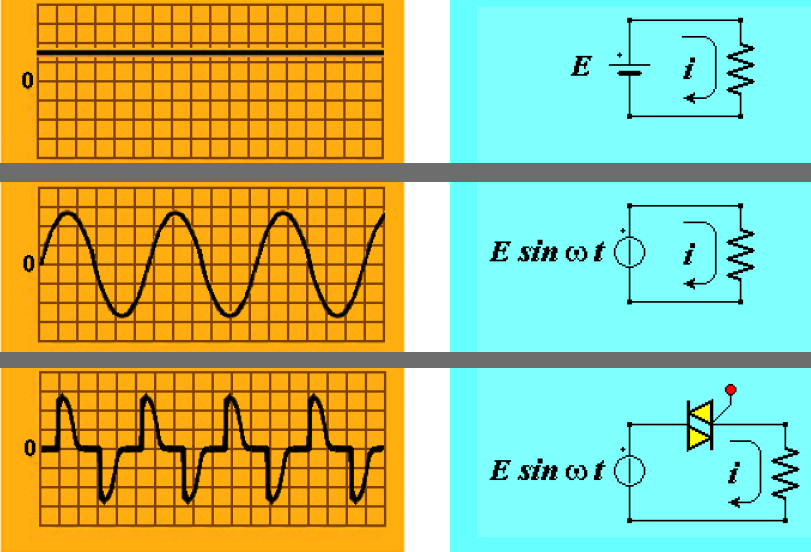
\includegraphics[scale = 0.8]{Confronto di tensioni in uscita e circuiti.PNG}
\end{figure}

Nel primo circuito, dato un generatore di tensione costante, in uscita (cioè ai capi del resistore) 
avremo una tensione costante, e che quindi rimane piatta. \newline 

In questo circuito, il valore efficace è la tensione costante. \newline 

Nel secondo circuito, dato un generatore di tensione periodico e sinusoidale, in uscita 
avremo una tensione che rimane periodica e sinusoidale. \newline 

In questo circuito, per calcolare il valore efficace, basta applicare il fattore di cresta $\sqrt{2}$. \newline 

Nel terzo circuito, dato un generatore periodico e sinusoidale, 
avremo questa forma d'onda non meglio nota. \newline 

In questo circuito, non possiamo applicare il fattore di cresta $\sqrt{2}$, 
bensì dovremo utilizzare degli strumenti $TRMS$, e che quindi calcolano o circuitalmente o digitalmente il valore efficace: 

{
    \Large 
    \begin{equation}
        I 
        = 
        \sqrt
        {
            \frac{1}{T}
            \int_{t_0}^{t_0 + T} 
            i^{2} (t) dt
        }
    \end{equation}
}

\newpage

\section{Strumenti RMS e TRMS}
\footnote{Slide della prof | SDME 4 Strumenti numerici indicatori - parte V | pag 16\\  
Appunti | 2025-05-09 | pag 4} 

Pratica da svolgere prima di utilizzare uno strumento di misura, è quello di visualizzare il segnale sull'oscilloscopio. \newline 

Per segnali che hanno andamento sinusoidale periodico, per calcolare il loro valore efficace possiamo utilizzare strumenti RMS, 
e che quindi calcolano, dal valore di picco della sinusoide, il valore efficace moltiplicando per $\frac{1}{\sqrt{2}}$. \newline 

Un esempio di tester RMS: 

\begin{figure}[h]
    \centering
    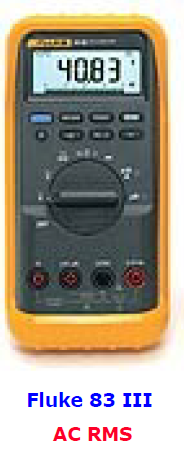
\includegraphics[scale = 0.8]{Fluke 83 III AC RMS.PNG}
\end{figure}

Invece, se il segnale presenta comportamenti non sinusoidali, per calcolare il valore efficace è meglio applicare il calcolo di valore efficace: 
questo si può fare utilizzando strumenti TRMS. \newline 

Esempi di tester TRMS: 

\begin{figure}[h]
    \centering
    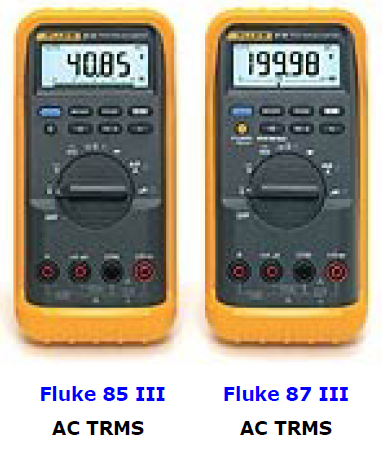
\includegraphics[scale = 0.8]{Strumenti Fluke TRMS.PNG}
\end{figure}

Gli strumenti TRMS sono più costosi, economicamente parlando, rispetto agli strumenti RMS perchè devono fare più conti e sono più complessi. \newline 

Si può utilizzare uno strumento TRMS per un segnale sinusoidale periodico, ma non avrebbe tanto senso (è come andare a fare la spesa con una Ferrari, meglio andarci in Pandino). \newline

\newpage 

\section{RMS - TRMS}
\footnote{Slide della prof | SDME 4 Strumenti numerici indicatori - parte V | pag 17\\  
Appunti | 2025-05-09 | pag 5}

Gli strumenti TRMS applicano circuitalmente il seguente calcolo: 

{
    \Large 
    \begin{equation}
        G 
        = 
        \sqrt
        {
            \frac{1}{T}
            \int_{t_0}^{t_0 + T} 
            g^{2} (t) dt
        }
    \end{equation}
}

dove g(t) è il valore istantaneo di una grandezza fisica, T il suo periodo, $t_0$ l'istante in cui si inzia la misura e G è il valore efficace. \newline 

Oppure, scritto in un'altra maniera, gli strumenti TRMS calcolano il valore efficace G di una grandezza periodica g(t) ed è 
la radice quadrata del valore medio sul periodo della grandezza al quadrato. \newline 

Gli strumenti che applicano questa formula sono strumenti a vero valore efficace: 
dall'inglese TRMS True Root Mean Square. \newline 

Gli strumenti che moltiplicano il valore massimo per $\frac{1}{\sqrt{2}}$ sono strumenti a quasi valore efficace: 
dall'inglese RMS Root Mean Square. \newline 

\newpage 

\section{TRMS / DC con calcolo del valore medio del quadrato del misurando}
\footnote{Slide della prof | SDME 4 Strumenti numerici indicatori - parte V | pag 18\\  
Appunti | 2025-05-09 | pag 5 | 2025-06-23 Ricevimento | pag 6, 8 }

Una possibile architettura di un circuito TRMS / DC è la seguente: 

\begin{figure}[h]
    \centering
    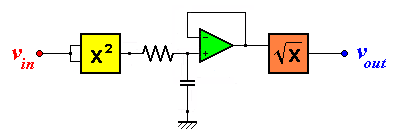
\includegraphics[scale = 2]{Architettura di TRMS DC.png}
\end{figure}

Riportando nuovamente il calcolo matematico da svolgere per il calcolo del valore efficace di una grandezza G: 

{
    \Large 
    \begin{equation}
        G 
        = 
        \sqrt
        {
            \frac{1}{T}
            \int_{t_0}^{t_0 + T} 
            g^{2} (t) dt
        }
    \end{equation}
}

Per una tensione V, diventa: 

{
    \Large 
    \begin{equation}
        V 
        = 
        \sqrt
        {
            \frac{1}{T}
            \int_{t_0}^{t_0 + T} 
            v^{2} (t) dt
        }
    \end{equation}
}

Se $v_{in}$ non ha un andamento periodico ogni tempo T, il valore efficace calcolato dalla seguente architettura sarà differente ogni tempo T. \newline

Iniziamo l'analisi del circuito (in figura partendo da sinistra verso destra). \newline 

Il blocco giallo $x^{2}$ eleva alla seconda $v_{in}$: 
quindi implementa il $v^{2} (t)$ matematico. \newline 

Dopo il blocco $x^{2}$, è presente un resistore e un condensatore, che in Fourier, sono un filtro passa basso; 
se il filtro presenta una frequenza di taglio $f_c$ molto bassa che tende a $\omega = 0$, nel tempo implementano il calcolo del valore medio, quindi l'integrale $\int_{t_0}^{t_0 + T} v^{2} (t) dt$ e la divisione per $T$. \newline 

L'amplificatore operazionale (triangolo verde) è presente in configurazione seguitore perchè ha guadagno 1 rispetto al segnale dopo il filtro passa basso , 
permette anche di pulire il segnale e dividere il circuito in due grazie al concetto di massa virtuale dell'amplificatore operazionale. \newline 

Dopo l'amplificatore operazionale, nel segnale viene calcolata la radice quadrata (blocchetto arancione con $\sqrt{x}$). \newline 

Alla fine in $v_{out}$ sarà calcolato il valore efficace V partendo da $v_{in}$. \newline 

Con questo tipo di architettura, il segnale $v_{in}$ può essere qualsiasi, e non per forza deve essere sinusoidale, ma deve essere periodico perchè il calcolo del valore medio dipende da T periodo del segnale di ingresso. \newline 

\newpage 

\subsection{Amplificatore logaritmico con OpAmp}
\footnote{Slide della prof | SDME 4 Strumenti numerici indicatori - parte V | pag 19 - 20\\  
Appunti | 2025-05-09 | pag 6 - 8, 9 | 2025-06-23 Ricevimento | pag 9 - 10}

Dall'analisi matematica 1, sappiamo che, grazie alle proprietà dei logaritmi: 

{
    \Large 
    \begin{equation}
        \begin{split}
            y &= \ln(x^{k})
            \\
            &\updownarrow
            \\ 
            y &= k \cdot \ln(x)
        \end{split}
    \end{equation}
}

e poi, per calcolare $x^{k}$ applichiamo l'operazione opposta, cioè quella dell'anti-logaritmo. \newline 

\begin{tcolorbox}
    Un piccolo ripasso di analisi matematica 1 sui logaritmi che non fa mai male, ricordando che ln è il logaritmo in base e: \\
    \url{https://www.youmath.it/lezioni/analisi-matematica/le-funzioni-elementari-e-le-loro-proprieta/84-proprieta-dei-logaritmi.html}   
\end{tcolorbox}

Partendo dal segnale $v_{in}$, da un punto di vista circuitale $y = \ln (x^{k})$  
può essere implementato con il seguente circuito: 

\begin{figure}[h]
    \centering
    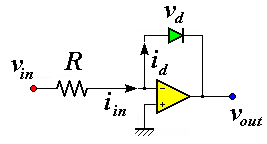
\includegraphics[scale = 2]{Amplificatore logaritmico con OpAmp.png}
\end{figure}

Grazie al concetto di massa virtuale dell'AmpOp: 

{
    \Large 
    \begin{equation}
        i_{in} = i_d
    \end{equation}
}

in cui: 

{
    \Large 
    \begin{equation}
        i_{in}
        = 
        \frac{v_{in}}{R}
    \end{equation}
}

Nel ramo tra la massa virtuale e $v_{out}$, 
siccome è presente un diodo, componente che ha un comportamento esponenziale, 
avremo che: 

{
    \Large 
    \begin{equation}
        i_d 
        = 
        i_0 \cdot e^{\frac{V_d}{k}}
    \end{equation}
}

dove $V_d$ è la tensione ai capi del diodo, k è il fattore scala del diodo e $i_0$ è la corrente di bias del diodo. \newline 

Per corrente di bias $i_0$ si intende una corrente che passa nel diodo anche se $v_d$ è nulla: quindi anche se il diodo non è polarizzato, passa una corrente di valore $i_0$. \newline 

Per questo motivo, nelle varie architetture, si cerca di diminuire se possibile la tensione ai capi di un diodo. \newline 

\newpage 

Da un punto di vista grafico: 

\begin{figure}[h]
    \centering
    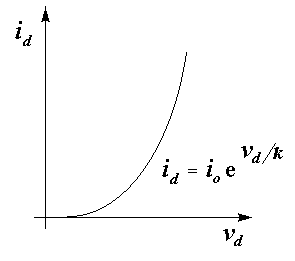
\includegraphics[scale = 1]{Relazione tra tensione e corrente in un diodo.png}
\end{figure}

Possiamo scrivere: 

{
    \Large 
    \begin{equation}
        \frac{i_d}{i_0}
        = 
        e^{\frac{V_d}{k}}
    \end{equation}
}

Applicando l'operatore inverso dell'esponenziale, cioè il logaritmo, ambo e due le parti, 
l'equazione diventerà: 

{
    \Large 
    \begin{equation}
        \ln(\frac{i_d}{i_0}) 
        = 
        \frac{v_d}{k}
    \end{equation}
}

Isolando $v_d$: 

{
    \Large 
    \begin{equation}
        v_d = k \cdot \ln(\frac{i_d}{i_0})
    \end{equation}
}

Da un punto di vista grafico: 

\begin{figure}[h]
    \centering
    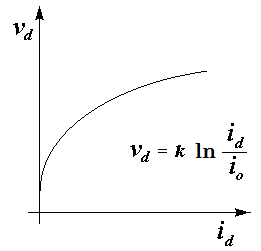
\includegraphics[scale = 1]{Relazione tra corrente e tensione in un diodo.png}
\end{figure}


Sapendo la relazione tra $i_d$ e $i_{in}$, possiamo semplificare $v_d$ come: 

{
    \Large 
    \begin{equation}
        \begin{split}
            v_d &= k \cdot \ln(\frac{i_d}{i_0})
            \\
            &\downarrow 
            \\
            v_d &= k \cdot \ln( \frac{v_{in}}{R} \cdot \frac{1}{i_0})
            \\
            & = k \cdot \ln(\frac{v_{in}}{R \cdot i_0})
        \end{split}
    \end{equation}
}

Quindi, alla fine di tutti questi conti, avremo che, sapendo che $v_d$ è uguale a $v_{out}$: 

{
    \Large 
    \begin{equation}
        \abs{v_{out}}
        = 
        k \cdot \ln(\frac{v_{in}}{i_0 \cdot R})
    \end{equation}
}

Per calcolarsi l'elevamento alla seconda $x^{k}$ non sono necessari tutti i punti della funzione logaritmo, 
bensì solo quella in cui $i_d = \frac{v_{in}}{R}$: 

\begin{figure}[h]
    \centering
    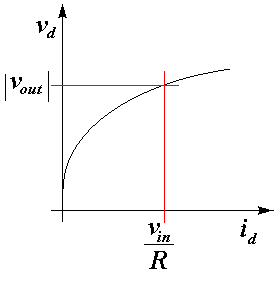
\includegraphics[scale = 1]{punto che ci interessa per l'uso dei logaritmi per l'elevamento alla potenza.png}
\end{figure}

Si considera $\abs{v_{out}}$, quindi il modulo di $v_{out}$ perchè non sappiamo il verso di $v_{in}$. \newline 

Se volgiamo calcolare l'elevamento alla seconda di $\frac{v_{in}}{R \cdot i_0}$, 
grazie alle proprietà dei logaritmo, possiamo scrivere: 

{
    \Large
    \begin{equation}
        \begin{split}
        \abs{v_{out}}
        &= 
        2 \cdot k \cdot \ln(\frac{v_{in}}{i_0 \cdot R})
        \\
        &= 
        k \cdot \ln(\frac{v_{in}}{i_0 \cdot R})^{2}
        \end{split}
    \end{equation}
}

e poi isolare l'argomento $(\frac{v_{in}}{i_0 \cdot R})^{2}$ da $\ln$, così da avere solo $(\frac{v_{in}}{i_0 \cdot R})^{2}$. \newline 

\newpage 

Per implementare questa nuova funzione di $\abs{v_{out}}$, dal circuito iniziale con un diodo, aggiungiamo un altro diodo al ramo tra massa virtuale e $v_{out}$: 

\begin{figure}[h]
    \centering
    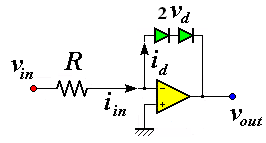
\includegraphics[scale = 2]{Amplificatore logaritmico alla seconda con OpAmp.png}
\end{figure}

Siccome il nostro obbiettivo è calcolarci l'elevamento alla seconda di $\frac{v_{in}}{R \cdot i_0}$ scegliamo: 

{
    \Large 
    \begin{equation}
        k = 1
    \end{equation}
}

Quindi $\abs{v_{out}}$ diventerà: 

{
    \Large 
    \begin{equation}
        \begin{split}
        \abs{v_{out}}
        &=  
        2 \cdot k \cdot \ln(\frac{v_{in}}{i_0 \cdot R})
        \\
        &\downarrow
        \\
        \abs{v_{out}}
        &=  
        2 \cdot 1 \cdot \ln(\frac{v_{in}}{i_0 \cdot R})
        \\
        &= 
        2 \cdot \ln(\frac{v_{in}}{i_0 \cdot R})
        \\
        &= 
        \ln(\frac{v_{in}}{i_0 \cdot R})^{2}
        \end{split}
    \end{equation}
}

Per calcolarsi il blocco $\sqrt{x}$ del TRMS / DC, 
possiamo utilizzare lo stesso circuito con resistore, un diodo e AmpOp ponendo: 

{
    \Large 
    \begin{equation}
        \begin{split}
            k &= \frac{1}{2}
            \\
            &\downarrow
            \\
            v_d &= k \cdot \ln(\frac{v_{in}}{i_0 \cdot R})
            \\
            &= 
            \frac{1}{2} \cdot \ln(\frac{v_{in}}{i_0 \cdot R})
            \\
            &= 
            \ln(\frac{v_{in}}{i_0 \cdot R})^{\frac{1}{2}}
            \\
            &= 
            \ln \sqrt{\frac{v_{in}}{i_0 \cdot R}}
        \end{split}
    \end{equation}
}

e poi calcolarci l'anti-logaritmo, come stiamo facendo con l'elevamento alla seconda. \newline 

\newpage 

\subsection{Amplificatore anti-logaritmico con OpAmp}
\footnote{Slide della prof | SDME 4 Strumenti numerici indicatori - parte V | pag 21\\  
Appunti | 2025-05-09 | pag 9}

Da: 

{
    \Large 
    \begin{equation}
        \abs{v_{out}}
        = 
        \ln(\frac{v_{in}}{i_0 \cdot R})^{2}
    \end{equation}
}

vogliamo isolare $(\frac{v_{in}}{i_0 \cdot R})^{2}$, 
quindi abbiamo bisogno di un circuito anti-logaritmo. \newline 

Una implementazione di circuito anti-logaritmo è la seguente: 

\begin{figure}[h]
    \centering
    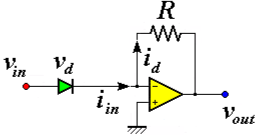
\includegraphics[scale = 2]{Amplificatore anti-logaritmico con OpAmp.png}
\end{figure}

che è lo stesso del circuito logaritmico ma in cui la posizione tra diodo e resistore è scambiata. \newline 

Se consideriamo $\abs{v_{out}}$ dall'amplificatore logaritmico il $v_{in}$ del circuito anti-logaritmico, 
$v_{out}$ sarà: 

{
    \Large 
    \begin{equation}
        \begin{split}
            \abs{v_{out}}
            &= 
            e^{v_{in}}
            \\
            &\downarrow
            \\
            \abs{v_{out}}
            &= 
            e^{\ln(\frac{v_{in}}{i_0 \cdot R})^{2}}
            \\ 
            &= 
            \left(\frac{v_{in}}{i_0 \cdot R}\right)^{2}
        \end{split}
    \end{equation}
}   

Ora che abbiamo visto una implementazione di $x^{2}$ possiamo visualizzare altri tipi di architetture per migliorare l'incertezza di misura ed essere più efficienti. \newline 

\newpage 

\section{TRMS/DC log-antilog}
\footnote{Slide della prof | SDME 4 Strumenti numerici indicatori - parte V | pag 22 - 27\\  
Appunti | 2025-05-09 | pag 9 - 11}

Un'altra architettura per applicare il calcolo del TRMS è la seguente: 

\begin{figure}[h]
    \centering
    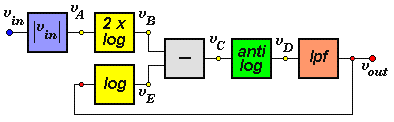
\includegraphics[scale = 2]{TRMS DC log antilog.png}
\end{figure}

Questo circuito implementa il calcolo del TRMS, quindi: 

{
    \Large 
    \begin{equation}
        v_{out} (t)
        =
        \sqrt{\frac{1}{T} \int_{t_0}^{t_0 + T} [v_{in} (t)]^{2}} dt
    \end{equation}
}

Nella realtà, nei multimetri tradizionali, viene implementato questo tipo di architettura piuttosto che quella precedente che abbiamo studiato, proprio perchè (anche se inizialmente sembra una cosa complicata) 
il ramo di retroazione permette di abbassare l'incertezza di misura. \newline 


Analizziamo bene il circuito. \newline 

Il blocco: 

{
    \Large 
    \begin{equation}
        v_A (t) 
        = 
        \abs{v_{in}} 
    \end{equation}
}

viene implementato perchè, come sappiamo dall'analisi matematica 1, il logaritmo non accetta argomenti minori di zero. \newline 

Dal punto di vista circuitale, il blocco $\abs{v_{in}}$ viene implementato con dei circuiti in cui sono presenti gli operazionali. \newline 

\begin{tcolorbox}
    Da: \\
    \url{https://www.dinfo.unifi.it/upload/sub/laboratori/uscnd/courses/applied-electronics/course-handouts/non-linear-applications-of-operational-amplifiers.pdf}
    pag 12 \newline 

    si può applicare questo circuito per svolgere il modulo di un segnale di ingresso: \\ 
    Raddrizzatore a Doppia semi-onda - Applicazione del Diodo di Precisione

    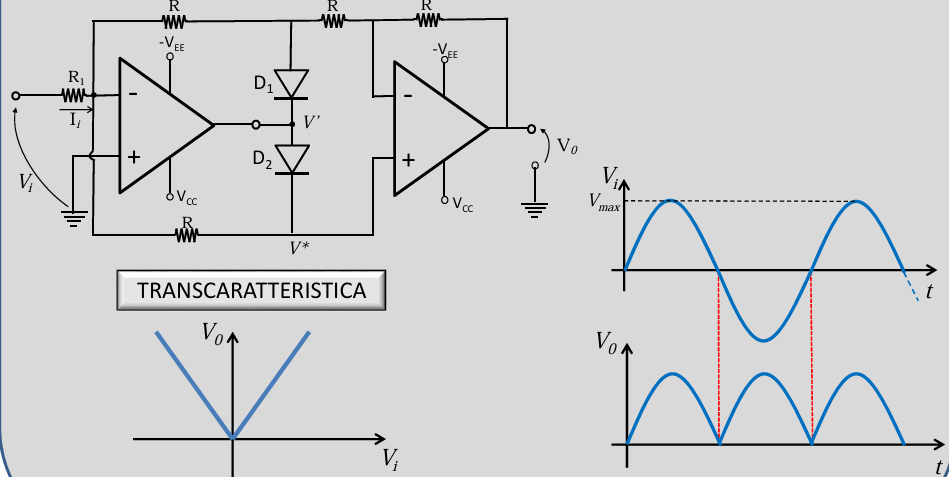
\includegraphics[scale = 0.8]{Raddrizzatore a Doppia semionda - applicazione del diodo di precisione.PNG}
    
\end{tcolorbox}

Passando al prossimo blocco dopo $v_A$, abbiamo $v_B$, in cui, partendo da $v_{in}$ e applicando le proprietà dei logaritmi: 

{
    \Large 
    \begin{equation}
        \begin{split}
            v_B 
            &= 
            2 \cdot \ln(v_A)
            \\ 
            &= 
            2 \cdot \ln [v_{in} (t)]
            \\ 
            &= 
            \ln [v_{in} (t)]^{2}
        \end{split}
    \end{equation}
} 

Per notazione matematica, il modulo, che è indispensabile per la funzione logaritmo che ha dominio positivo, 
può essere tolto quando elevo l'argomento al quadrato, per le proprietà dei logaritmi. \newline 

Dalla tensione $v_B$ passiamo a $v_E$ dove:

{
    \Large 
    \begin{equation}
        v_E = \ln[v_{out}(t)]
    \end{equation}
}

Grazie al ramo di retroazione che collega $v_{out} (t)$, $v_E$ può essere calcolato in questa maniera. \newline 

Ancora non sappiamo quanto vale $v_{out}$, ma simbolicamente possiamo annotarla con questa notazione. \newline 

Ora passiamo al nodo $v_c$ dove, applicando le proprietà dei logaritmi, avremo che la differenza diventa una divisione:

{
    \Large 
    \begin{equation}
        \begin{split}
            v_c (t)
            &= 
            v_B (t) - v_E (t)
            \\
            &=
            \ln[v_{in} (t)]^{2} - \ln[v_{out} (t)]
            \\
            &= 
            \ln
            \frac{[v_{in} (t)]^{2}}{v_{out} (t)}
        \end{split}
    \end{equation}
}

Da $v_C$ passiamo al nodo $v_D$ dove è presente un blocco anti-log, quindi:

{
    \Large 
    \begin{equation}
        \begin{split}
            v_D (t)
            &= 
            e^{v_C}
            \\
            &= 
            e^{\ln \frac{[v_{in} (t)]^{2}}{v_{out} (t)} }
            \\
            &= 
            \frac{[v_{in} (t)]^{2}}{v_{out} (t)}
        \end{split}
    \end{equation}
}

$v_D (t)$ passa poi in un filtro passa basso (dall'inglese lpf Low Pass Filter), 
il quale ha frequenza di taglio talmente bassa da eliminare tutte le componenti alternate e mantenere solo la continua, 
che è la costante $\omega = 0 $ ed è pari al valore medio del segnale. \newline 

Quindi, dopo che è passato dall'lpf, avremo $v_{out} (t)$ che è al valore medio di $v_D (t)$, che, applicando la definizione di valore medio di $v_D (t)$ in un periodo T: 

{
    \Large 
    \begin{equation}
        \begin{split}
        v_{out} (t)
        &= 
        \overline{v_D (t)}
        \\
        &=
        \frac{1}{T}
        \int_{t_0}^{t_0 + T}
        \frac{[v_{in} (t)]^{2}}{v_{out} (t)} dt
        \end{split}
    \end{equation}
}

Se $v_{out} (t)$ è costante in $[t_0, t_0 + T]$ allora, si può portarlo dall'integrale, 
e svolgendo altri passi algebrici: 

{
    \Large
    \begin{equation}
        \begin{split}
        v_{out} (t) 
        &=
        \frac{1}{T}
        \int_{t_0}^{t_0 + T}
        \frac{[v_{in} (t)]^{2}}{v_{out} (t)} dt
        \\
        &\downarrow
        \\
        v_{out} (t) 
        &=
        \frac{1}{T}
        \frac{1}{v_{out} (t)}
        \int_{t_0}^{t_0 + T}
        [v_{in} (t)]^{2} dt
        \\
        [v_{out} (t)]^{2} 
        &=
        \frac{1}{T}
        \int_{t_0}^{t_0 + T}
        [v_{in} (t)]^{2} dt
        \\
        \sqrt{[v_{out} (t)]^{2}} 
        &=
        \sqrt
        {
        \frac{1}{T}
        \int_{t_0}^{t_0 + T}
        [v_{in} (t)]^{2} dt
        }
        \\
        v_{out} (t)
        &=
        \sqrt
        {
        \frac{1}{T}
        \int_{t_0}^{t_0 + T}
        [v_{in} (t)]^{2} dt
        }
        \end{split}
    \end{equation}
}

Per giustificare l'estrazione di $v_{out} (t)$ dal segno dell'integrale, 
operata nel passaggio precedente, deve essere valida l'ipotesi che il valore efficace della grandezza di ingresso si mantenga costante all'interno di un periodo. \newline

La $v_{out} (t)$ ottenuta è proporzionale al valore efficace di $v_{in} (t)$, 
qualunque sia la sua forma d'onda, 
nell'ipotesi che il suo spettro sia contenuto nella banda passante di tutti i blocchi presenti nella catena circuitale. \newline 

Per questo ultimo motivo, ecco perchè negli strumenti dove viene calcolato il TRMS del segnale di ingresso viene indicato il range di frequenza della grandezza da misurare. \newline 

\begin{tcolorbox}
    Nelle pagine della presentazione della prof da 28 a 30 sono indicati dei modelli disponibili in commercio di integrati che calcolano il TRMS e RMS, 
    le diverse architetture, ma soprattutto, la relazione tra minore incertezza e aumento dei costi economici dell'integrato
\end{tcolorbox}

\newpage 

\section{Voltmetro per DC e AC}
\footnote{Slide della prof | SDME 4 Strumenti numerici indicatori - parte V | pag 31 - 35\\  
Appunti | 2025-05-09 | pag 12 - 13}

Come accennato negli scorsi capitoli, il tester, o altri strumenti numerici odierni, fisicamente sono lo stesso strumento, ma svolgono funzioni molteplici. \newline 

Riportando l'architettura di un voltmetro in DC a quattro portate: 

\begin{figure}[h]
    \centering
    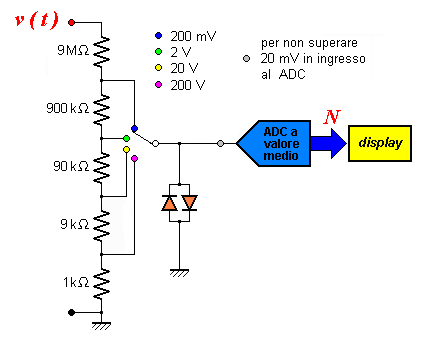
\includegraphics[scale = 1]{voltmetro numero con rete resistiva adattatore di livello.png}
\end{figure}

possiamo adattarlo a voltmetro sia in AC che per DC utilizzando un nuovo selettore e un convertitore RMS/DC (o TRMS/DC in base al segnale da misurare): 

\begin{figure}[h]
    \centering
    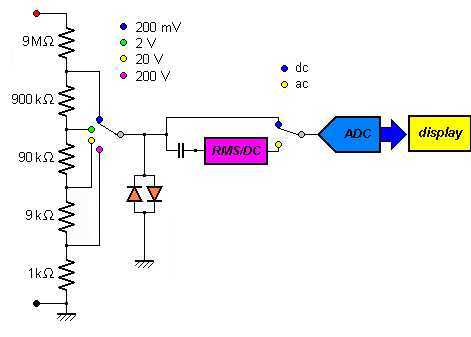
\includegraphics[scale = 1.5]{voltmetro numero con rete resistiva adattatore di livello e RMS-DC.png}
\end{figure}

Il condensatore prima del blocco RMS/DC toglie la componente continua del segnale, cioè quella a $\omega = 0$. \newline 

\newpage

Se il segnale sotto misura presente sia una componente continua, che una componente in AC come il seguente segnale: 

\begin{figure}[h]
    \centering
    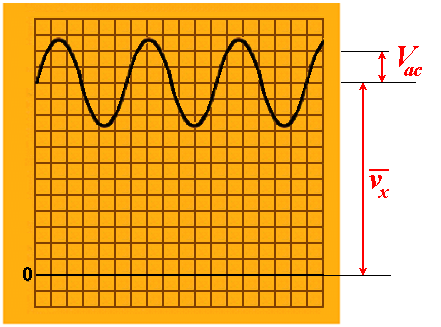
\includegraphics[scale = 1]{Segnale in AC con offset.png}
\end{figure}

per il calcolare il valore efficace $V_x$: 

\begin{enumerate}
    \item mettere il selettore del voltmetro in DC per calcolare $\overline{v_x}$ che è il valore in continua del segnale a $\omega = 0$
    \item cambiare il selettore del voltmetro in AC, e avremo il valore efficace $V_{ac}$ di tutte le altri componenti del segnale tranne la continua  
\end{enumerate}

Se è presente un blocco RMS/DC si presuppone che il segnale abbia solo una componente e sia sinusoidale periodica. \newline 

Se è presente un blocco TRMS/DC si presuppone che il segnale può avere qualsiasi forma, anche non lineare, per il calcolo del valore efficace $V_{ac}$. \newline 

Il valore del segnale: 

{
    \Large
    \begin{equation}
        v_x(t)
        = 
        \overline{v_x}
        + 
        v_{p, x} \sin(\omega t)
    \end{equation}
}

Il valore efficace di $v_x$ è: 

{
    \Large
    \begin{equation}
        V_x
        = 
        \sqrt{\overline{v_x}^{2} + V_{ac}^{2}}
    \end{equation}
}

Da un punto di vista grafico $V_x$ possiamo vederlo come l'ipotenusa di un triangolo rettangolo: 

\begin{figure}[h]
    \centering
    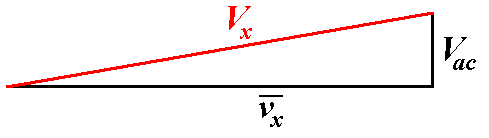
\includegraphics[scale = 1]{Valore efficace di un segnale sinusoidale con offset.png}
\end{figure}

Calcolando l'incertezza alla formula $V_x$, essendo una grandezza calcolata indirettamente, 
dobbiamo calcolare la propagazione delle incertezze di $v_x$ e $V_{ac}$ su $V_x$. \newline 

Avremo che l'incertezza $\Delta V_x$ di $V_x$ è: 

{
    \Large 
    \begin{equation}
        \Delta V_x
        = 
        \frac{V_{ac} \cdot \Delta V_{ac} + \overline{v_x} \cdot \Delta \overline{v_x}}{V_x}
    \end{equation}
}

Sapendo come è fatto il segnale, $V_{ac}$ è molto basso rispetto a $V_x$, quindi anche se $\Delta V_{ac}$ è molto grande, 
un numero molto grande moltiplicato per un numero molto piccolo, da un fattore molto piccolo. \newline 

Invece, $\overline{v_x}$ è molto alto, ma sapendo che lo strumento è stato progettato per lavorare in DC ed opera nelle migliori condizioni, 
$\Delta \overline{v_x}$ sarà molto basso: come prima, un valore molto grande, moltiplicato per un valore molto piccolo, da un valore molto piccolo. \newline 

Di conseguenza, in $\Delta V_x$, un denominatore piccolo, diviso per un numeratore grande, avrà un contributo piccolo. \newline 

Se invece con questo strumento volessimo misurare il valore efficace della tensione alternata $v_{ac}$, cioè $V_{ac}$: 

{
    \Large 
    \begin{equation}
        V_{ac}
        = 
        \sqrt{V_x ^{2} - \overline{v_x}^{2}}
    \end{equation}
}

o in figura: 

\begin{figure}[h]
    \centering
    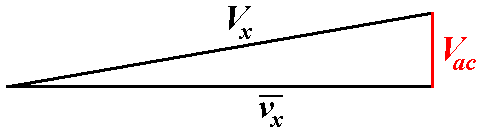
\includegraphics[scale = 1]{Calcolo del ripple con un voltmetro DC accoppiato in AC.png}
\end{figure}


L'incertezza $\Delta V_{ac}$ sarà uguale a: 

{
    \Large 
    \begin{equation}
        \Delta V_x 
        =
        \frac{V_x \cdot \Delta V_x + \overline{v_x} \cdot \Delta \overline{v_x}}{V_{ac}}
    \end{equation}
}

$V_x$ e $\Delta V_x$ sono fattori molto alti, $\overline{v_x}$ e $\Delta \overline{v_x}$ sono generalmente molto bassi, 
quindi avremo un nominatore molto grande diviso per un fattore $V_{ac}$ molto piccolo. \newline 

Quindi $\Delta V_x$ sarà un fattore molto grande. \newline 

Grazie a queste spiegazioni è possibile dire perchè il condensatore serve a farci misurare il valore efficace della sola componente alternata. \newline 

Lo strumento si chiama AC perchè funziona sfruttando l'accoppiamento in alternata dello stadio di ingresso e di quello di misura (Alternate Coupling). \newline

\newpage 

